\documentclass[10pt]{article}
\usepackage[utf8]{inputenc}
\usepackage[a4paper, total={12cm, 22cm}]{geometry} % MARGIN 15.5 instead of 14 was initial

\usepackage{comment} 

\usepackage{hyperref}

\usepackage{float}
\usepackage{graphicx}

\usepackage[dvipsnames]{xcolor}
\usepackage[normalem]{ulem}

\setlength\parindent{0pt}
\setlength{\parskip}{2em}

\usepackage{amsmath}
\usepackage{listings}
\usepackage{comment}
\usepackage{longtable}
\usepackage{markdown}

\usepackage{biblatex}
\addbibresource{bibliography.bib}


% FOOTER AND HEADER %
\usepackage{etoolbox}
\usepackage{fancyhdr}
\pagestyle{fancy} 
\newcommand{\frontmatter}{\clearpage \cfoot{\thepage\ }
\fancyhead{}
\renewcommand{\headrulewidth}{0pt}
\setcounter{page}{1}
\pagenumbering{Roman}}
\newcommand{\mainmatter}{\clearpage \cfoot{\thepage\ of \pageref{LastPage}}
\fancyhead[LE,RO]{Group I}\fancyhead[RE,LO]{\leftmark}
\renewcommand{\headrulewidth}{0.4pt}
\setcounter{page}{1}
\pagenumbering{arabic}}
\newcommand{\backmatter}{\clearpage \cfoot{\thepage\ }
\fancyhead{}
\renewcommand{\headrulewidth}{0pt}
\setcounter{page}{1}
\pagenumbering{alph}}
\patchcmd{\chapter}{\thispagestyle{plain}}{\thispagestyle{fancy}}{}{}
% Front page background %
\usepackage[
firstpage=true,
opacity=0.25,
angle=0,
]{background}
\backgroundsetup{contents={
\includegraphics[scale=0.1]
{images/background.jpg}}}



\begin{document}

\begin{titlepage}
    \begin{center}
        \vspace*{1cm}

        \Huge
        \textbf{Exam Report}
        
        \vspace{0.5cm}
        
        \Large
        Group I
            
        \vspace{1.5cm}
         
        \textbf{Christian Skovsgaard Rieck (crie@itu.dk)}
        \textbf{Daniel Stokholm Thomsen (dant@itu.dk)}\\
        \textbf{Harpa Gudrún Hreinsdóttir (hahr@itu.dk)}
        \textbf{Johan Fritze Neve (jone@itu.dk)}
            
        \vspace{1.5cm}
        
       
            
        \vfill
            
        DevOps, Software Evolution and Software Maintenance\\
         KSDSESM1KU
            
        \vspace{0.8cm}
            
        
\includegraphics[width=0.4\textwidth]{images/ITU_logo_UK.jpg}
            
        \Large
        Department of Computer Science\\
        Denmark\\
        1st of June 2022
            
    \end{center}
\end{titlepage}

\frontmatter
\tableofcontents

\mainmatter

\section{Introduction}
This report covers various aspects of Group I's project in the course, DevOps, Software Evolution and Software Maintenance. The most important artefacts of the project are listed with their respective link in appendix \ref{alllinks}.

\section{System's perspective}

\subsection{Architecture and Design}
% Probably need package module view and c&c, especially the sequence diagram for interactions with subsystems
The system is a mini-version of Twitter, called MiniTwit.
The system has two main packages, a Blazor frontend and a ASP.NET Core API. The API and Frontend decisions are described in detail in sections \ref{frontenddisc} \& \ref{apidisc}, respectively. The overall decision log can be found on \href{https://github.com/Arklaide/devopsITUproject/blob/main/report/sub-reports/decision_log.md}{our GitHub Repository}. See Fig. \ref{fig:package} for the package module view. The architectural views have been created based on the 3+1 model proposed by Christensen et al\cite{christensen20163+}.

\begin{figure} [H]
  \centering
  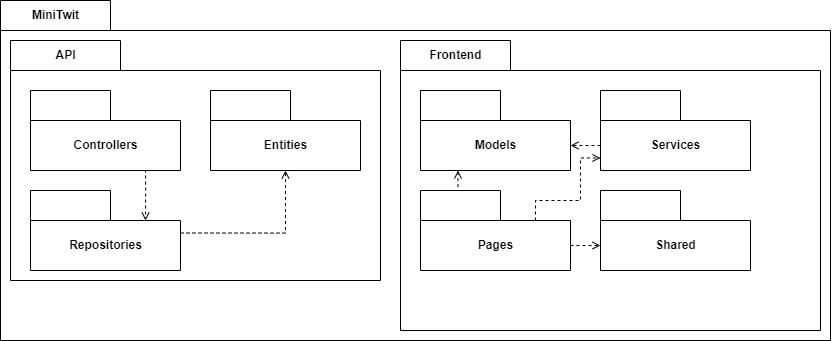
\includegraphics[width=0.9\textwidth]{images/devops-overall_module_view.png}
  \caption{Package diagram}
  \label{fig:package}
\end{figure}

The system relies on various other services. The system uses ElasticSearch and Kibana for logging and Prometheus and Grafana for monitoring. The system is depicted in an overall context diagram in Fig. \ref{fig:context}. The six mentioned services are part of a docker stack swarm, which is managed by one docker swarm manager machine and supported by one docker swarm worker machine. The system, specifically the API, interacts with a managed database system. The database and the two machines are located and hosted in DigitalOcean.

\begin{figure} [H]
  \centering
  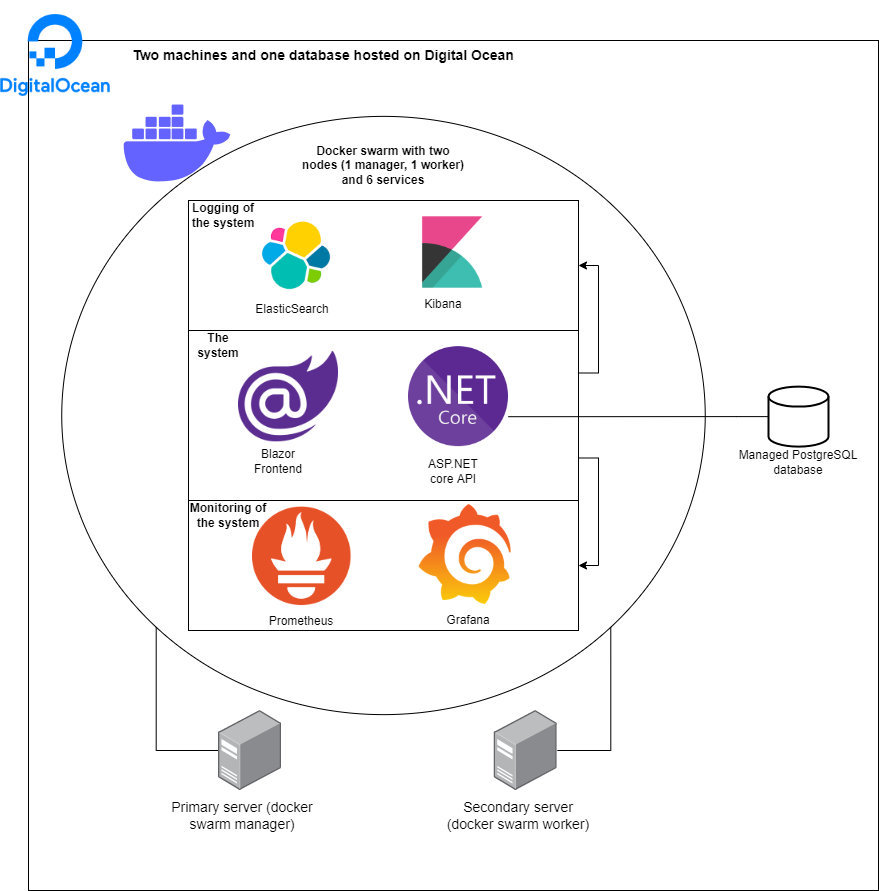
\includegraphics[width=0.9\textwidth]{images/devops-diagram.png}
  \caption{Context diagram}
  \label{fig:context}
\end{figure}

The Component \& Connector view can be seen in Fig. \ref{fig:cc}, which shows how the different components of the system are connected. The greyed out components are external but are included to provide a better overview of how the system has been used in this project.

\begin{figure} [H]
  \centering
  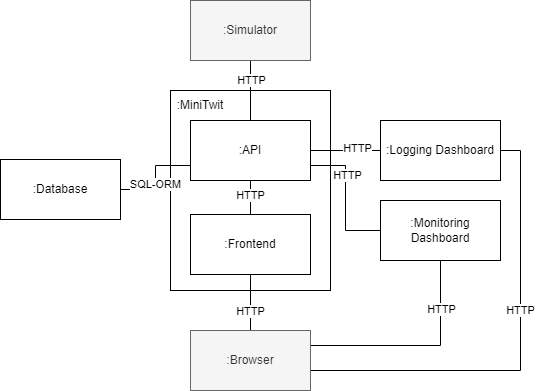
\includegraphics[width=0.9\textwidth]{images/devops-cc.png}
  \caption{Component \& Connector view}
  \label{fig:cc}
\end{figure}

An example of the interactions of subsystems can be seen in the sequence diagram in Fig. \ref{fig:sequence}. The example revolves around a user registration, and shows two scenarios, one where a user already exists and one where the user does not exist. The two scenarios return different status codes and communicate differently with the logging and monitoring components.

\begin{figure} [H]
  \centering
  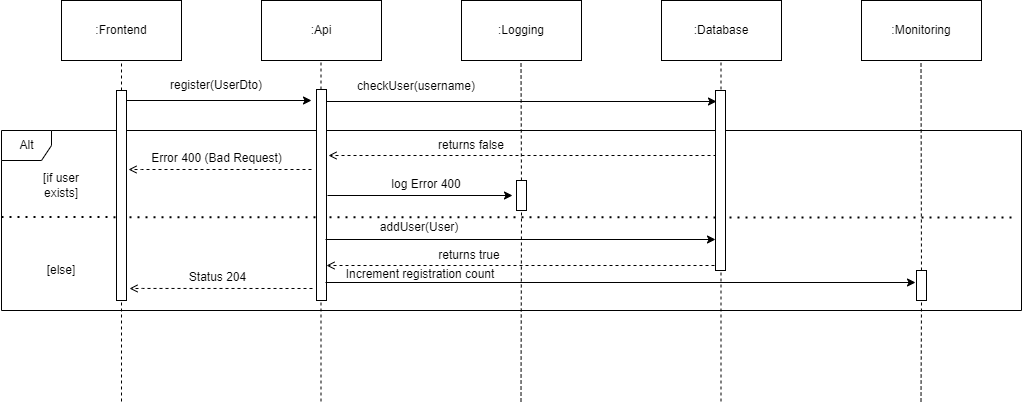
\includegraphics[width=0.9\textwidth]{images/devops-sequence.png}
  \caption{Sequence diagram}
  \label{fig:sequence}
\end{figure}

The deployment view of the system can be seen in Fig. \ref{fig:deloy}. The different entities are as follows:

\begin{itemize}
    \item \texttt{Digital Ocean Managed DB:} PostgreSQL database responsible for storing user data, following data and twits hosted on Digital Ocean. Kept separately from the servers to ensure backups and a less error-prone environment for data storage.
    \item \texttt{Primary Server:} Ubuntu server responsible for managing the docker swarm.
    \begin{itemize}
        \item \texttt{API:} ASP.NET Core API is responsible for communicating between the Frontend and database, acting as our backend.
        \item \texttt{Frontend:} Blazor Frontend provides a user interface to view and create twits.
        \item \texttt{Prometheus:} Providing metrics for monitoring with default Prometheus metrics and custom metrics for the API. The choice of Prometheus is based on industry standards.
        \item \texttt{Grafana:} Monitoring dashboard based on metrics from Prometheus to provide business and technical insight into the running system. The choice of Grafana is based on industry standards.
        \item \texttt{ElasticSearch:} Search for the aggregation of our logs sent from the application. 
        \item \texttt{Kibana:} A dashboard showing the logs aggregated in ElasticSearch.
    \end{itemize}
    \item \texttt{Secondary Server:} Ubuntu server responsible for being a docker swarm worker and hosting the docker instances requested by the manager.
\end{itemize}

\begin{figure} [H]
  \centering
  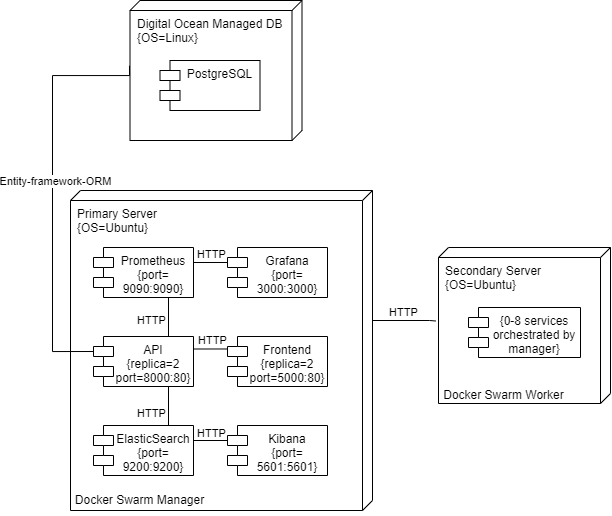
\includegraphics[width=0.9\textwidth]{images/devops-deployment.png}
  \caption{Deployment view}
  \label{fig:deloy}
\end{figure}

\subsubsection{Frontend}
\label{frontenddisc}

The reasons why we decided to go with Blazor are based on the following factors:
\begin{enumerate}
\item It is convenient to use the same language pack for both the frontend and API
\item Simple routing, HttpClient and Dependency Injection
\end{enumerate}

To store the state of the logged-in user we decided to go with a State class, which contains private functions to update the authentication state. When the state is changed it notifies the dependant classes (which have injected the State class). 

\subsubsection{API}
\label{apidisc}
We have chosen to do the API using ASP.NET Core using the shared data pattern. There are several reasons why we chose this stack:
\begin{enumerate}
    \item Endpoints are automatically serialized to properly formatted JSON, which is being used in our frontend, as well as the simulator.
    \item URl-Routing is done inline easily, as well as query parameters and request bodies, are automatically bound to method parameters
    \item Logging of database interactions is automatically added. When we set up the ESK-stack\footnote{ElasticSearch-Serilog-Kibana}, we have to only do minor additions to have meaningful logging in our entire application.
    \item Entity Framework Core makes it easy to communicate with our database and is the base for the shared data architectural pattern choice.
\end{enumerate}
\subsection{Dependencies}
The direct dependencies of the API and Frontend are visualized as a graph in Fig. \ref{fig:depgrapg}. The graph shows us that the API has 16 dependencies and the Frontend has 7.
\begin{figure} [H]
  \centering
  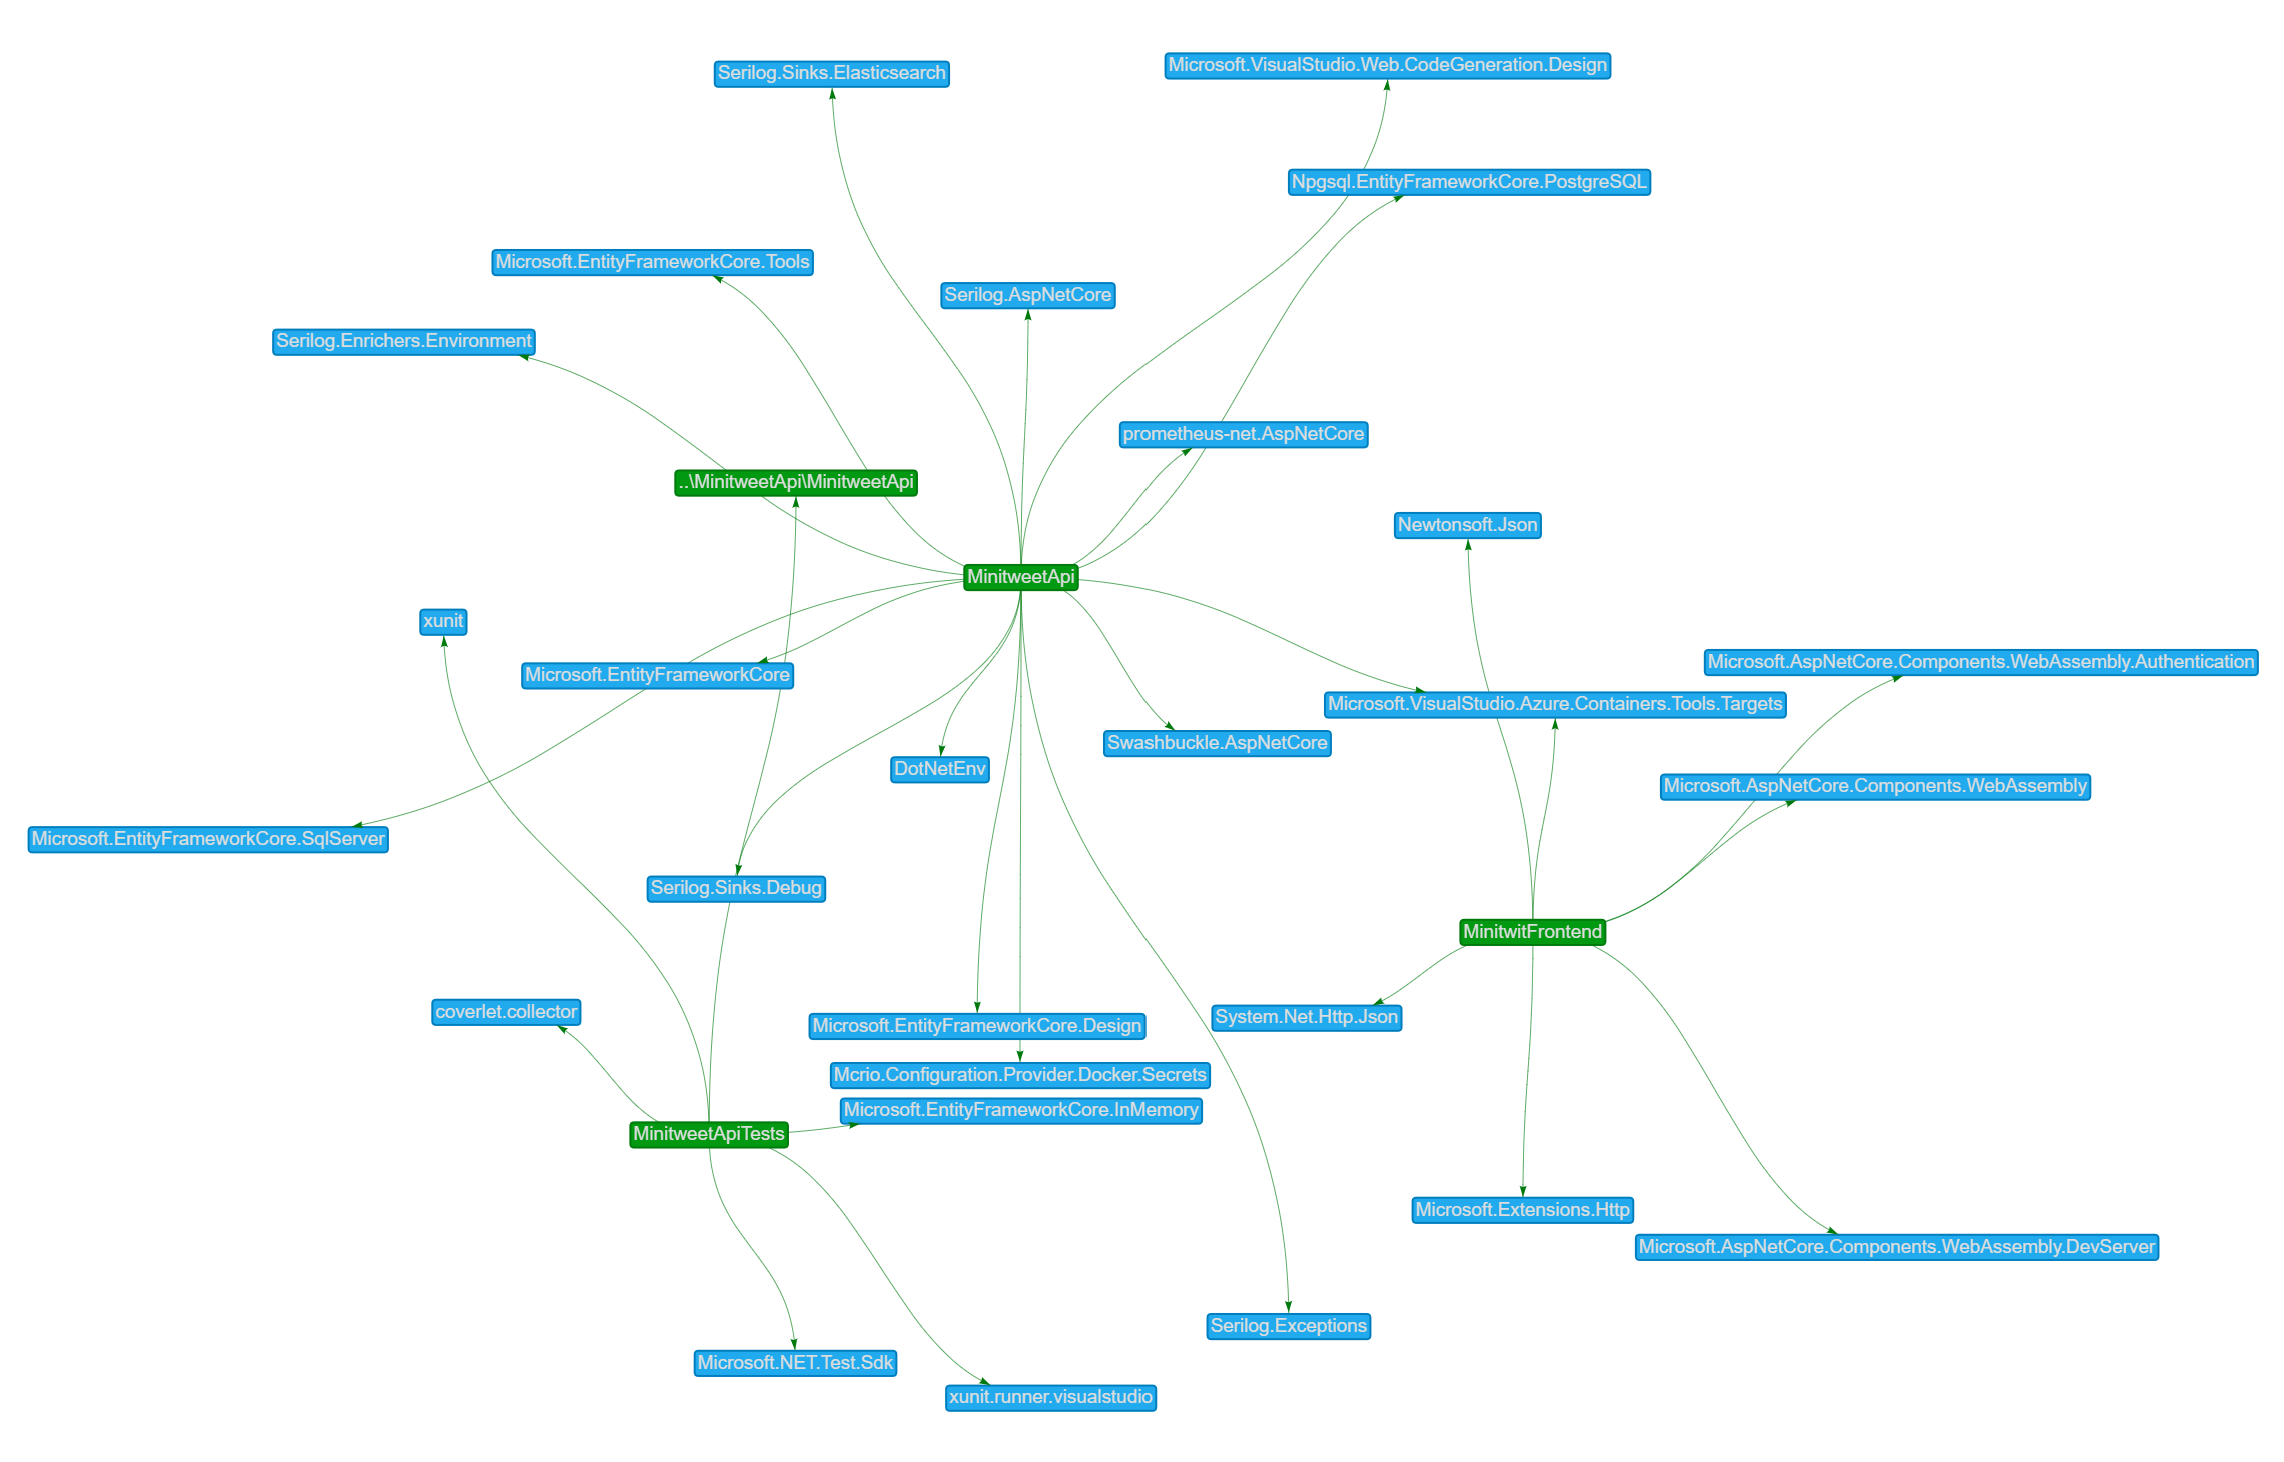
\includegraphics[width=0.9\textwidth]{images/dependencygraph.png}
  \caption{Dependency Graph}
  \label{fig:depgrapg}
\end{figure}

There are multiple other dependencies of the project, we depend on multiple GitHub actions in our workflows, such as SSH and checking code out. There are also dependencies in our docker images, such as \texttt{nginx:alpine} for the Frontend image. Furthermore, our servers besides having standard Ubuntu dependencies, have \texttt{docker.io} \& \texttt{doctl} as dependencies. Lastly, we depend on Terraform for infrastructure as code. An overview can be seen in Fig. \ref{fig:otherdep}.

\begin{figure} [H]
  \centering
  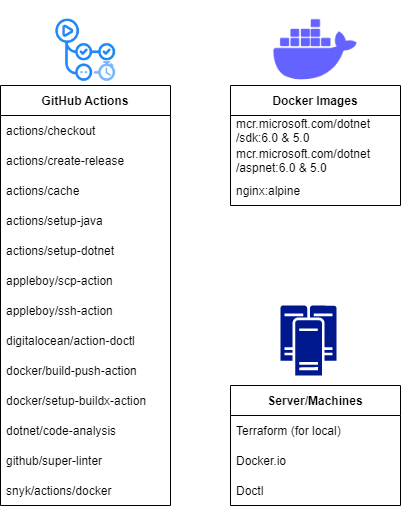
\includegraphics[width=0.7\textwidth]{images/devops-otherdependencies.png}
  \caption{Other dependencies overview}
  \label{fig:otherdep}
\end{figure}

An extensive list of all direct dependencies of this project, their name, description, and license can be found in appendix \ref{depappendix}.


\subsection{Current state of the systems}
The current state of the artefacts in the repository is summarized below, the state is found with different tools.
The state as analyzed by Better Code Hub can be seen in Fig. \ref{fig:bch}, it shows 8/10 checks look good, however, automatic testing and short units of code are not passed. Another static analysis tool places our system in category C, which means there is 10-20\% technical debt and they estimate it will take one week to clear out the debt. Moreover, the technical debt relates to 11 cases of code smells and 12 cases of code duplication. However, Sonar Cloud shows a better technical debt of less than 5\%, but a lower reliability score due to bugs. The Sonar Cloud state can be seen in Fig. \ref{fig:sc}. The overall state of the system is acceptable, but it opens up for various maintenance needs.

\begin{figure} [H]
  \centering
  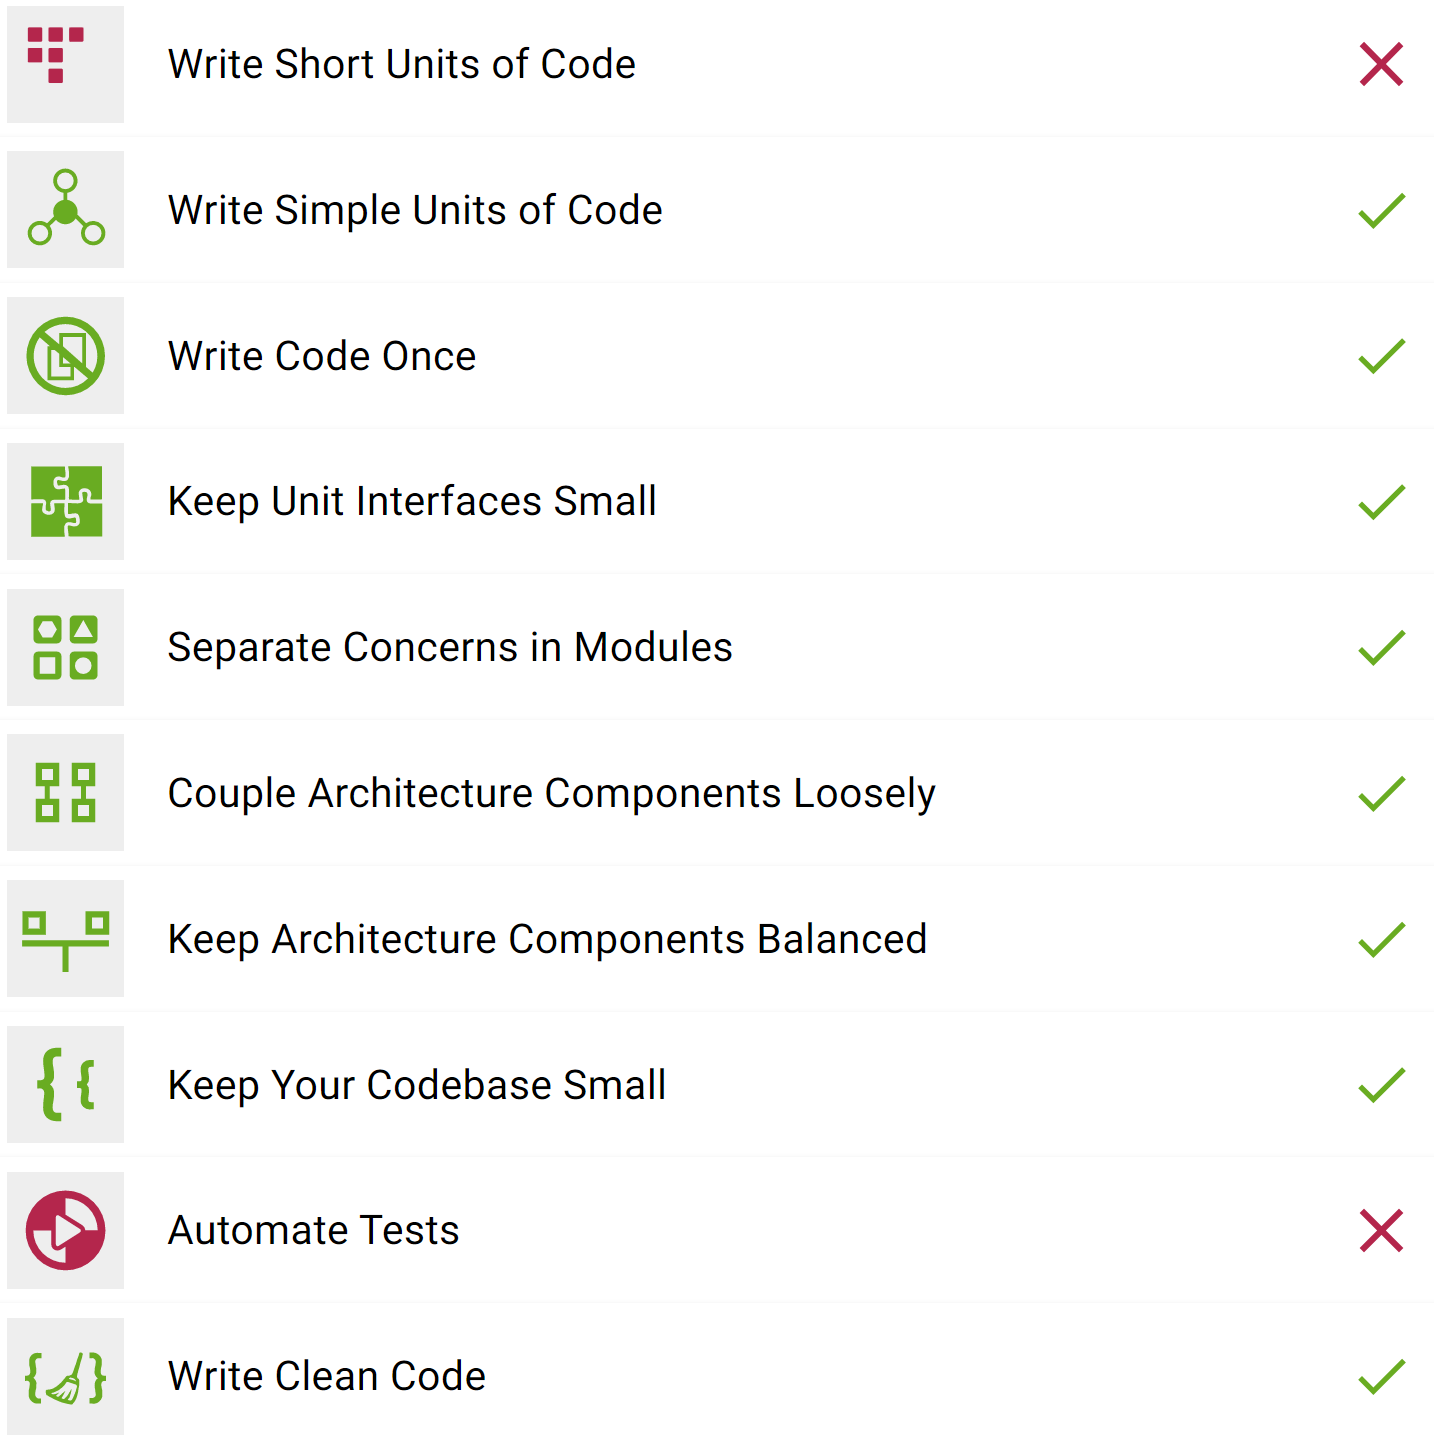
\includegraphics[width=0.9\textwidth]{images/bettercodehub.png}
  \caption{Better Code Hub state results}
  \label{fig:bch}
\end{figure}

\begin{figure} [H]
  \centering
  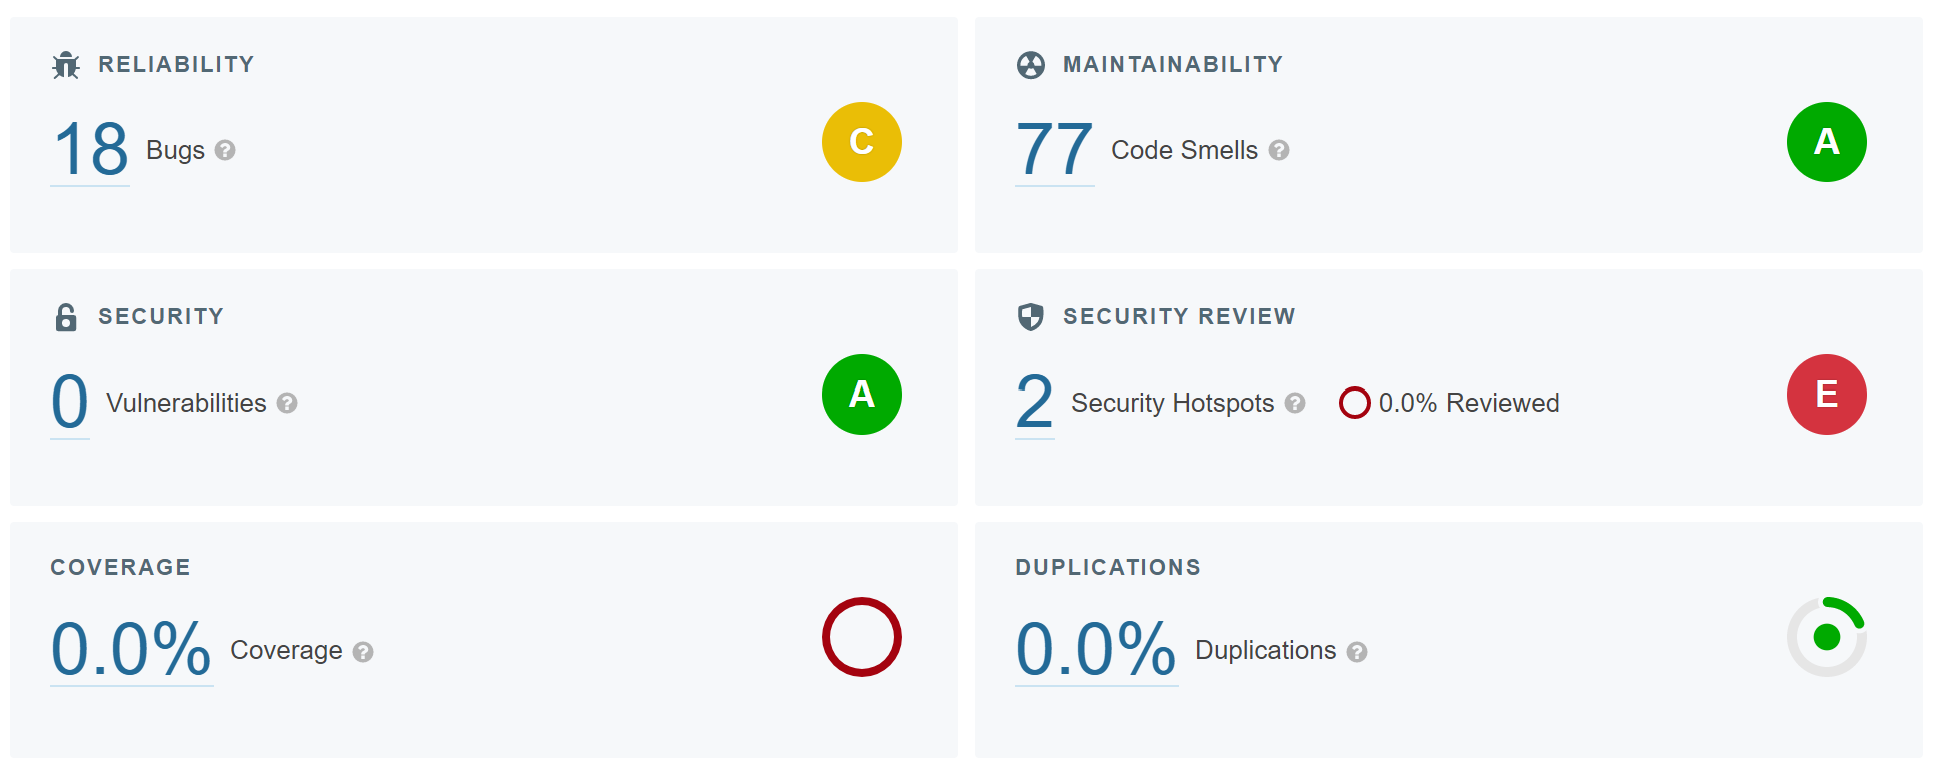
\includegraphics[width=0.9\textwidth]{images/sonarcloud.png}
  \caption{Sonar Cloud state results}
  \label{fig:sc}
\end{figure}


\subsection{Licenses}
We are using a MIT license which is a permissive, free, and open source license. The choice of the license is due to wanting to support the open-source community and thereby not restricting the use. All of our direct dependencies are using either MIT or Apache 2.0, which are both permissive licenses. That makes our MIT license compatible with all of our direct dependencies.

\section{Process' perspective}
% Add general stuff think 3ways (+ contributions?)
% https://github.com/Arklaide/devopsITUproject/blob/main/report/sub-reports/ThreeWays.md
%How do you interact as developers?
%How is the team organized?
We have aimed to adhere to the \textit{"Three Ways"} as described in \textit{"The DevOps HandBook"}\cite{kim2021devops}. A summary of our use of the three ways is described below, the initial internal notes concerning it can be found on our \href{https://github.com/Arklaide/devopsITUproject/blob/main/report/sub-reports/ThreeWays.md}{GitHub repository}.
A key task has been to simplify release to production in order to accommodate hotfixes and avoid big-bang releases. We use the GitFlow branching strategy together with, a Kanban board, and a streamlined CI/CD pipeline. The CI/CD pipeline is visualized in section \ref{cicdchain}. The Kanban board is described in section \ref{Development_process}. In the kickoff phase of the project, we spent some time adjusting expectations to help establish psychological safety. Furthermore, we try to have shared responsibility for the work by doing code reviews.

\subsection{Organization of Repository}
We chose to version control all our code and files as a mono-repository on GitHub. The repository can be viewed here: \href{https://github.com/Arklaide/devopsITUproject}{DevopsITUproject}.
Every project has its own folder. However, the two main projects, the Frontend and the API, share a .NET solution file, which is located in the root of the repository.
We chose this option because we want to keep the number of repositories as low as possible, and also this makes our lives easier when working with the application since a change in the API often triggers some code changes to the Frontend and vice versa and therefore simpler to keep them in the same repository.

\subsection{Branching strategy}
We have been using the branching model known as GitFlow. This effectively means that we have a main branch for releases and a develop branch for development/testing. We avoid the extra step of making a release branch and merge directly to main from develop for simplicity. An alternative could have been Trunk-based, but since we were not experienced in DevOps, we chose to make it more strict, another important reason is that the repository is public and open for contributions. The contributions guidelines can be found on our \href{https://github.com/Arklaide/devopsITUproject/blob/main/contributing.md}{GitHub repository}. The workflow consists of the developer branching out from develop and after finishing their feature, they will do a pull request from their respective branch to the develop branch, where they have to assign at least one reviewer. When we are ready for a release, we create a PR from develop to main and once that is approved, our GitHub Action will automatically deploy the artefacts to DigitalOcean, and our newly improved system will be in production. A visualization of the branching strategy in action can be seen in Fig. \ref{fig:branch}.

\begin{figure} [H]
  \centering
  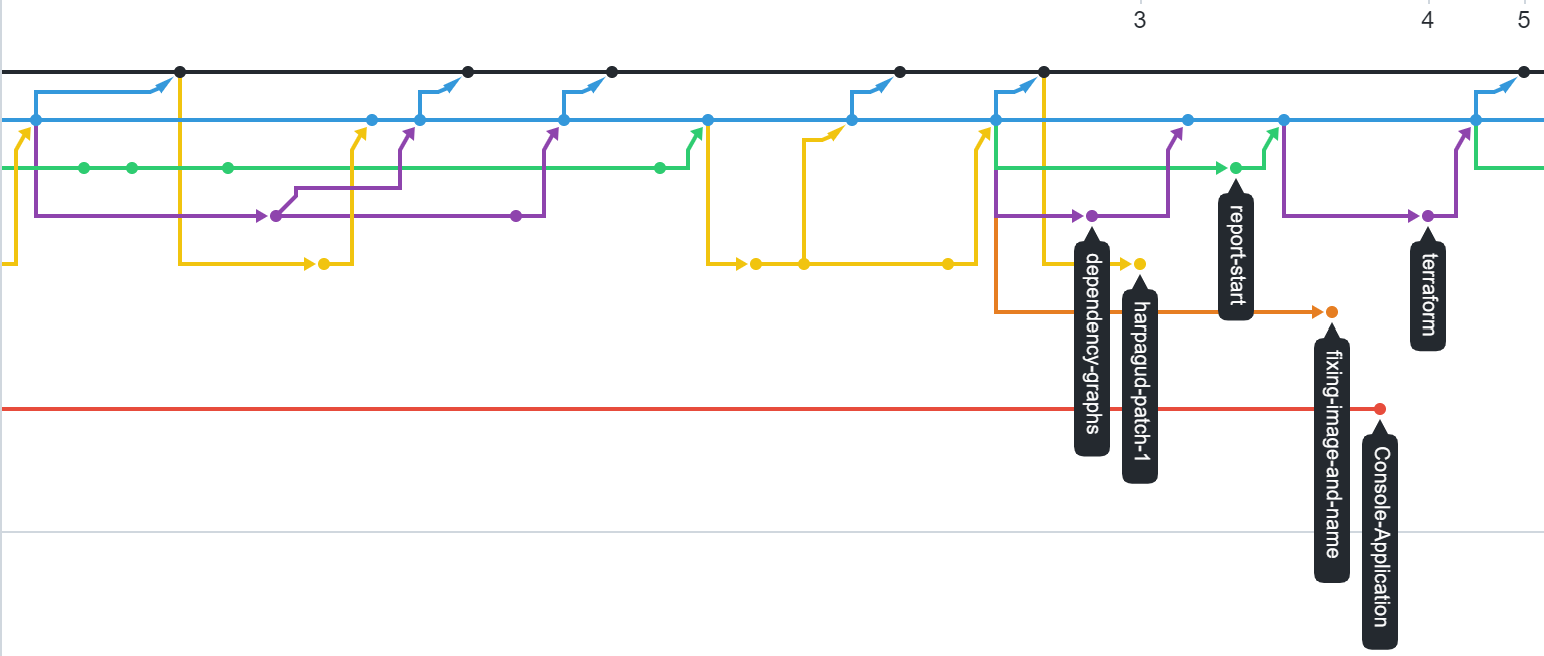
\includegraphics[width=0.9\textwidth]{images/branch.png}
  \caption{Branching visualization}
  \label{fig:branch}
\end{figure}

\subsection{CI/CD chain}
\subsubsection{Flow of the CI/CD chain}
\label{cicdchain}
Fig. \ref{fig:flow} is a visualization of the entire process from a developer's idea, to it being pushed to production.

\begin{figure}[H]
    \centering
    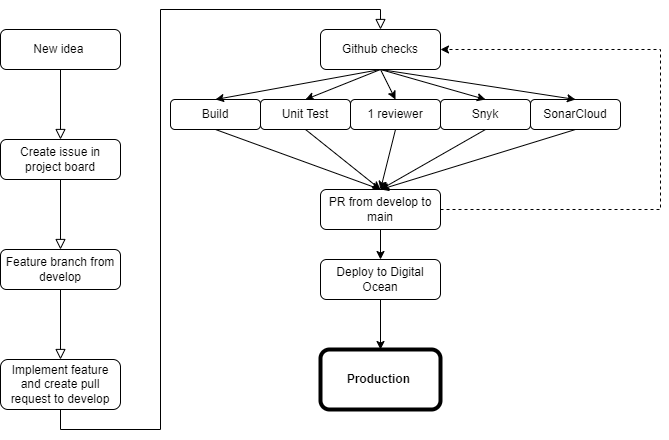
\includegraphics[width=\textwidth]{images/flow.PNG}
    \caption{CI/CD flow}
    \label{fig:flow}
\end{figure}

\subsubsection{Releases}
To ensure we have regular releases, we have set up GitHub actions that auto release. One of them does a biweekly release and the other one does a release on pushes to the main branch. The GitHub actions can be found at the following links:
\begin{enumerate}
    \item \href{https://github.com/Arklaide/devopsITUproject/blob/main/.github/workflows/releaseonpush.yml}{Release on pushes to main}
    \item \href{https://github.com/Arklaide/devopsITUproject/blob/main/.github/workflows/autorelease.yml}{Biweekly release}
\end{enumerate}

\subsubsection{Pull Request}
To ensure some consistency and quality in our code we have added various checks that validate our code when creating a pull request, these are:
\begin{enumerate}
    \item The API and Frontend are buildable and unit tests are run
    \item SonarCloud Code Analysis
    \item Better Code Hub
    \item Code Climate
    \item Snyk vulnerability scanning
\end{enumerate}
\subsubsection{Deployment}
We have automated our deployment to production using a GitHub action: 
\href{https://github.com/Arklaide/devopsITUproject/blob/main/.github/workflows/deploy.yaml}{\textit{deploy action}}.
This action will trigger on every push to the main branch and will publish our system on our servers. The action includes some checks, namely .NET code analysis, Snyk Docker image scan, unit tests, and linting of the codebase. The state of the checks is described in the \href{https://github.com/Arklaide/devopsITUproject/blob/main/report/sub-reports/decision_log.md}{decision log}.


\subsection{Development process}
\label{Development_process}
%Applied development process and tools supporting it
To have an overview of all issues and a platform to distribute and assign these, we have decided to use GitHub Project Board.
The board is divided into categories, and each issue is assigned one of the following categories:
\begin{enumerate}
    \item \texttt{Brainstorm/Ideas}: Where we keep track of new ideas.
    \item \texttt{Todo}: Where we keep our issues that need to be done in the future.
    \item \texttt{In Progress}: Here we keep our issues we are currently working on - We try to limit our work in progress to work in small batches to increase productivity. This also helps us in avoiding context switching, since we try to focus on one issue at a time.
    \item \texttt{Code review}: Here we keep our issues which are to be code reviewed before merging to the develop branch.
    \item \texttt{Ready for release}: Here we keep our issues which are approved and waiting in develop to be merged for a release to main.
    \item \texttt{Done}: Here we keep our issues which are done and deployed to main.
\end{enumerate}
Each issue also has an assigned person. Combined with the status of the issues, we have a neat overview of open tasks.
\\
\\
The overview can be seen in Fig. \ref{fig:Kanban}


\begin{figure}[h]
    \centering
    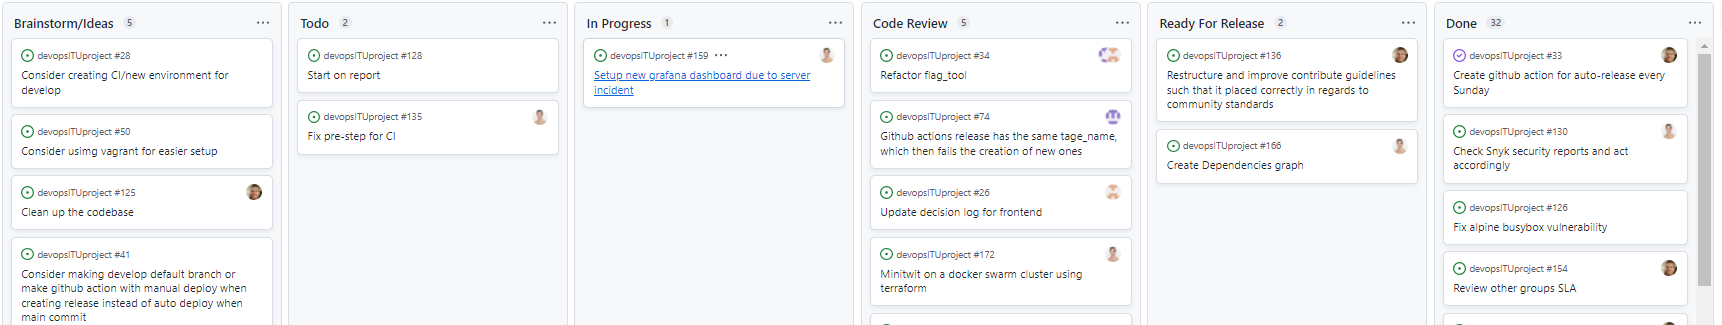
\includegraphics[width=\textwidth]{images/Kanban.PNG}
    \caption{GitHub Project Board}
    \label{fig:Kanban}
\end{figure}

\subsection{Monitoring}
%How do you monitor (graphana/promitheus)
We are using Prometheus and Grafana as the monitoring platform for our application. There is a ASP.NET Core package\footnote{https://www.nuget.org/packages/prometheus-net.AspNetCore/} for Prometheus so it is easy for us to incorporate this into our system.

%What exactly do you monitor
We monitor several metrics in our system. The business metrics are:
\begin{enumerate}
    \item The number of registered users since the last release
    \item The number of times users that have logged in to our system since the last release 
\end{enumerate}
These are metrics which can be used by the business responsible to measure the growth and size of our application or if a new update is well received. The business metrics can be seen in Fig. \ref{fig:monitoring}. 

\begin{figure}[H]
    \centering
    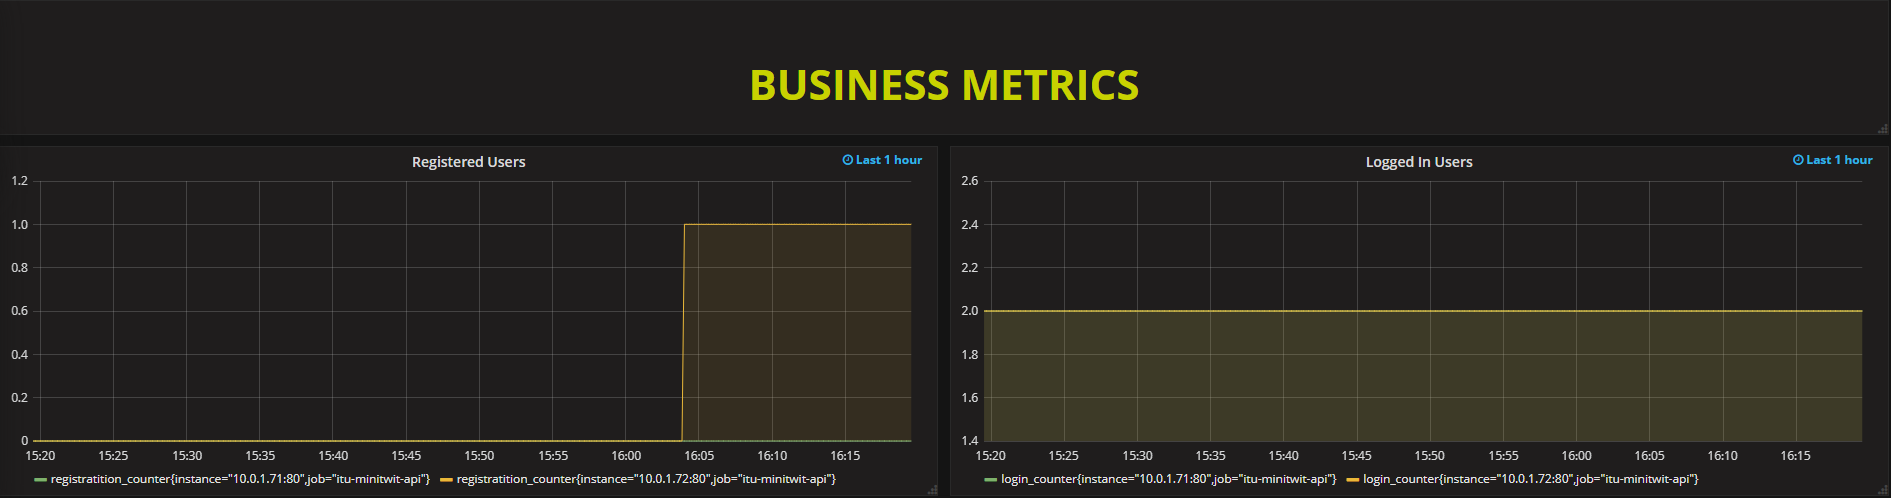
\includegraphics[width=\textwidth]{images/monitoringbusiness.PNG}
    \caption{Business metrics visualized from Grafana}
    \label{fig:monitoring}
\end{figure}

The monitoring also includes technical metrics that can help with server/system maintenance, these are:
\begin{enumerate}
    \item The total user and system CPU time spent
    \item The amount of http requests to our application
    \item Occupied memory
\end{enumerate}

\begin{figure}[h]
    \centering
    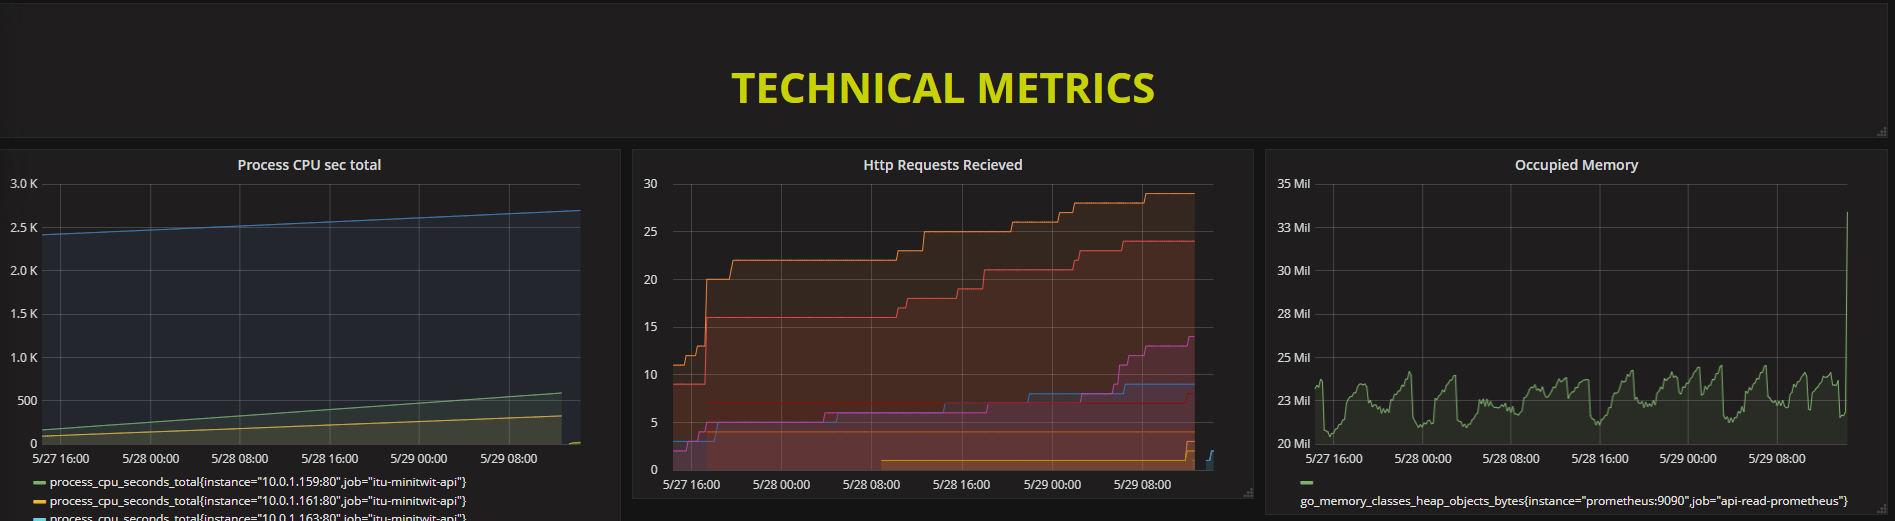
\includegraphics[width=\textwidth]{images/monitoring technical.PNG}
    \caption{Technical metrics visualized from Grafana}
    \label{fig:monitoringtechnical}
\end{figure}

\subsection{Logging}
%What do we log
We have decided to use the logging as is in Entity Framework. This means that every time our applications send a command to the database, whether it is inserts, updates, or deletes, it is being logged. This means that all interactions with the API are being logged, and since the Frontend mostly consists of API requests, we have a transitive logging relation to the Frontend.    
%how do we aggregate logs
\\
\\
We have decided to use a variation of the popular EFK-stack which is a logging aggregation ecosystem. First of all, we use Serilog, which is a .NET logging library, to get all of our logging information sent to ElasticSearch. We then use Kibana to better query and visualize the data stored in the ElasticSearch database. We then have the possibility to filter the data on a lot of criteria which can give us good troubleshooting capabilities.

An example of the visualization of the logging can be seen in Fig. \ref{fig:logging_visualization}:
\begin{figure}[H]
    \centering
    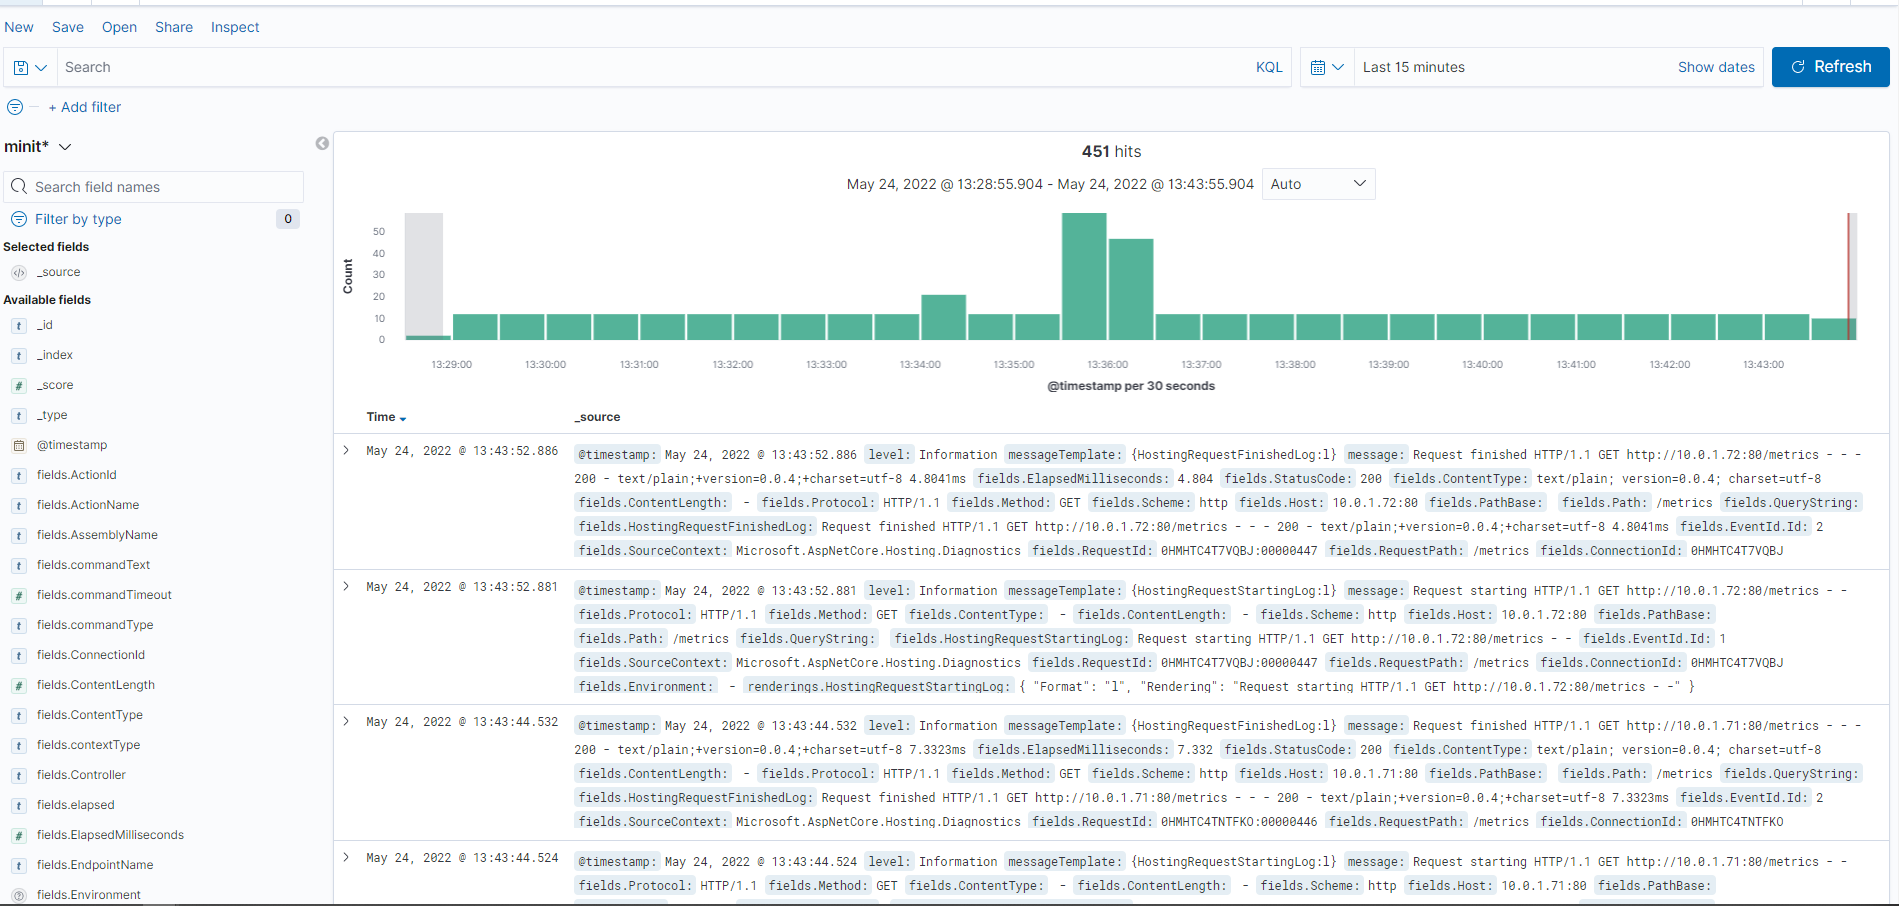
\includegraphics[width=\textwidth]{images/loggingvisualization.PNG}
    \caption{Logging visualization}
    \label{fig:logging_visualization}
\end{figure}

\subsection{Security assessment}
The system has been assessed with regards to security with two automatic penetration testing tools and a manual penetration testing. The whole security assessment report can be found in \href{https://github.com/Arklaide/devopsITUproject/blob/main/report/sub-reports/SecurityAssessment.md}{Our GitHub Repository}, this summary contains references found only there. The results are as follows:

\begin{itemize}
    \item Metasploit WMAP on Kali has been run and it shows no vulnerabilities
    \item Skipfish on Kali has been run and it shows nothing important, but indicates missing charset
    \item The user info API endpoint sends the password in plain text (everyone can see this). This is broken access control and relates to risk no 6.
    \begin{itemize}
        \item The hashing of the passwords seems broken
        \item It is possible to use this data to log in as other users
    \end{itemize}
\end{itemize}

The actions points based on the results are:
\begin{itemize}
    \item Implement countermeasure for risk no 6
    \begin{itemize}
    \item Ensure proper salting, hashing and authentication 
    \item Ensure proper endpoint security
    \item Ensure no unnecessary data is sent as responses
    \end{itemize}
    \item Switch from HTTP to HTTPS for enhanced security
\end{itemize}

Furthermore, OWASP\footnote{https://owasp.org/} includes insufficient logging and monitoring as a security risk. The current state of our logging is acceptable since it is possible to manual see some results from the penetration test, such as tools trying to access config sub-sites. However, nothing is automatic. Furthermore, the monitoring does not give much information, other than a few technical and business-related metrics, such as the numbers of logins. The security issue concerning risk no 6 that was found, can't be seen with the current logging/monitoring.

\subsection{Critical incident}
The group lost access to the first server of the project. It was no longer possible to log in via SSH-keys or in the DigitalOcean UI. The server was put in recovery mode, but access was still not possible to obtain even when resetting the root password. The solution was to quickly deploy new servers, but now with two machines using Docker Swarm. The downtime was about 4 hours mostly due to creating a better setup with Docker Swarm and little manual configuration of the servers. It was not possible to find any suspicious activity, moreover, there was no extra load on the CPU or other metrics of the server, which indicates that no one has installed a BitCoin miner or other types of software that exploits our server. The root cause was never found, so the best corrective measure is to create the infrastructure as code. We now have support for Terraform, but this was not implemented at the time of the incident. The full incident report can be found on  \href{https://github.com/Arklaide/devopsITUproject/blob/main/report/sub-reports/incident_log.md}{our GitHub repository}.

Moreover, the incident can clearly be seen on the graph in Fig. \ref{fig:latest}, which shows how many requests our API accepts at specific times. There are notable drops, the two first being lack of a green-blue deployment strategy. The third and biggest is our server incident, due to lack of updating the API URL for the simulator even though the actual downtime was only 4 hours. The last drop is simply the end of the simulator.

\begin{figure} [H]
  \centering
  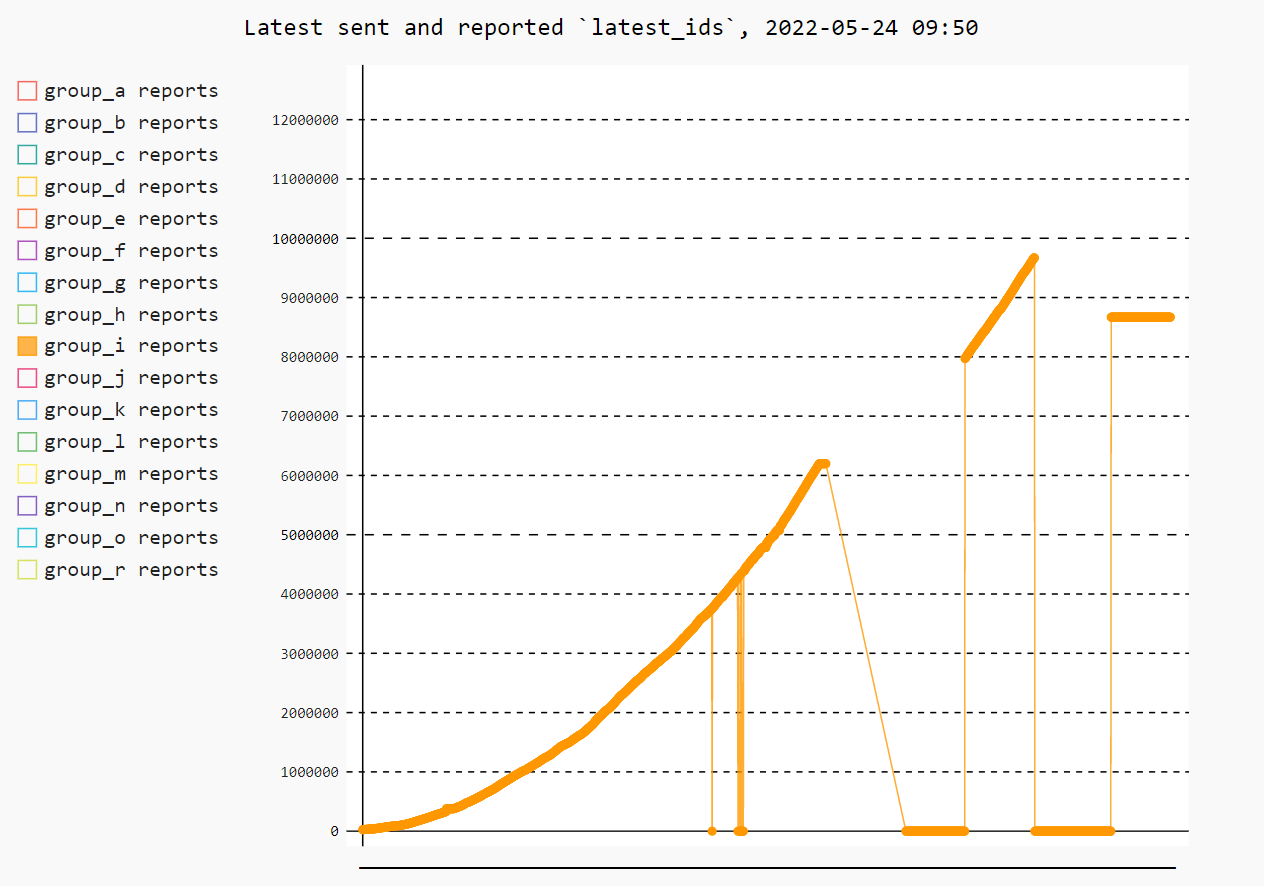
\includegraphics[width=0.9\textwidth]{images/latestids.PNG}
  \caption{Number of accepted API request over time}
  \label{fig:latest}
\end{figure}

\subsection{Scaling and load balancing}
The initial scaling was vertical since the logging service used up all the CPU, and more resources were needed. However, to avoid having a single point of failure, horizontal scaling was added via two machines and replicas for Docker containers.
The scaling and load balancing is set up with Docker Swarm. We have six Docker Services as a Docker Stack, two of them have two replicas, the API and Frontend. The scaling is static with Docker Swarm and more replicas are not created during higher loads. The Docker Swarm has one manager and one worker node. The manager is responsible for load balancing with the default Ingress routing load balancer. However, having only one manager node is a single point of failure, and in a real setup, there should be more managers and workers to ensure smooth operation. The deployment uses the Blue-Green strategy to ensure that a new upgrade starts before the current one stops, and then it shifts the load to the new one when it is ready. However, it is important to note that the database is not included in this strategy, which could yield problems if there are migrations to the database in the update.

\section{Lessons Learned Perspective}
%General lessons learned from devops %
There are numerous reflections on incorporating a DevOps style compared to previous development projects, these include:
\begin{itemize}
\item \textbf{Emphasize automation}. Building automation into the development life-cycle is critical to ensure that the software releases are consistent. Also, it allows the programmers to be liberated from less significant and time-consuming tasks to focus on processes that require more thinking and creativity.
\item \textbf{Using Docker}. Docker makes it easier to build and run the code in any setup to avoid on-boarding hassles for developers. This was even more empathized in the beginning before docker was added to the project, since developers were using different versions of .NET and different operating systems.
\item \textbf{Static analysis of codebase}. Using different static analysis tools helps determine areas to improve in the codebase, which could have been left unnoticed otherwise.
\end{itemize}

%evolution and refactoring
\subsection{Evolution and refactoring}

\textbf{Refactoring the database using Object–Relational Mapping}\\
A lesson that we can take along with us is the fact that we can utilize a lot of support given by the programming languages and its associated framework and libraries. When we were first given the task to refactor the python code, we chose to do it using .NET (reasons described in \ref{apidisc}), here we were given the complete SQL schema, we could then have used the effective scaffolding of the Entity Framework, to efficiently create all the model classes and the database context using the existing database. The issue regarding this can be seen at: \href{https://github.com/Arklaide/devopsITUproject/issues/11}{Issue 11}
\subsection{Operation}

\textbf{Importance of following separation of concerns when hosting on multiple servers}\\
One of the lessons we learned during the project, is the importance of separating concerns when writing code that is to be hosted on different servers. This came to importance when we were implementing logging.
We are using a logging library, Serilog, and when we configured it we had to connect to the right ElasticSearch database. We had to make sure it worked in test before deploying it to production. However, since our test environment is different from our production, the ideal solution would be to do the configuration in a higher level of abstraction, meaning that we never have to hard code the IPs of the servers we are connecting to. Not having this abstraction leads to a wide range of commits. Staring with \href{https://github.com/Arklaide/devopsITUproject/commit/30149bd9f5b1696ac1e10e3e6806d8db11e16c26}{commit 30149bd} and ending with \href{https://github.com/Arklaide/devopsITUproject/commit/686ee3893fabcce450d1844bf1743780d690413a}{commit 686ee38}
The ticket relating to these commits can be seen here: \href{https://github.com/Arklaide/devopsITUproject/issues/61}{\textit{Add Logging to the System}}
Luckily this issue was resolved but took a significant amount of time, which could have been spent more wisely.

\textbf{Difficulties testing operation and configuration leads to many fails and commits}\\
An important lesson concerned the configuration of automation of workflows, like the GitHub Action used to deploy the latest main branch to Digital Ocean. Operations and configuration are hard to test, the deploy action can only be tested by actually deploying to production. This led to many small commits in order to adjust when the action failed. It would have been nice to have a similar setup for the develop branch, such that the configuration could be tested without affecting production. A develop environment was not prioritised due to the costs associated. An example is on the 14th of March, when there were around 20 consecutive commits to try and fix the deployment of the system. Everything from missing nginx in the docker image to serve the static contents of the Blazor frontend and including environment variables in the deploy action. It starts with \href{https://github.com/Arklaide/devopsITUproject/commit/3cd6a117458ed81d38d57dfeb5b15afc5e4b69f5}{commit 3cd6a11} and ends with \href{https://github.com/Arklaide/devopsITUproject/commit/11e7e21605977232ae87d0dc9dddf2ac9f25cb8f}{commit 109eb16}.

%maintenance
\subsection{Maintenance}

\textbf{Cleaning old code to ensure a clean codebase}\\
An important part of a software life cycle is maintenance, correcting faults and improving the existing design. This also goes for our application. One of the things that is in need of cleaning is the file and folder structure of our code. As the application grows there is quite a big chance that the folder structure should evolve with it. However, taking the time and effort to do so, should be of a higher prioritization than what we have done in the project.
However, it is very difficult to find the time to go back and optimize when we have to stay ahead of the curve with the deadlines of the following week. 
These were addressed in the  \href{https://github.com/Arklaide/devopsITUproject/issues/125}{issue 125} this has sadly been lying dormant for a long time.
But for coming projects, we clearly see the value of having a clean base to develop upon.

\section{Future work}
There are various artefacts of the system that could have an improved setup, these are, but are not limited to:
\begin{itemize}
    \item ElasticSearch hosted on its own machines to avoid the logs being dependent on the same server as the API. Moreover, the heavy load of ElasticSearch won't affect the other services.
    \item Better monitoring and logging to ensure better security and traceability. Especially alerts when something seems off.
    \item Add file change policy to CI/CD pipeline to avoid building unnecessary parts and speed up the process
    \item Enforce quality gates and check requirements both for pull requests and the deployment GitHub action to ensure overall quality
    \item Add an extra environment as Production but for the develop branch. A development/testing environment could help to avoid problems and coding/configuring in the dark. This, however, could slow the deployment, but ensure better quality assurance.
\end{itemize}

\label{LastPage}

\backmatter 
\printbibliography

\newpage

\appendix
\section{Dependencies of the project}
\label{depappendix}
Below is a list of all the dependencies we are using in our project. Some of them have a strike-through which means we did not end up using them but they are currently still in our solution. One of the part of the maintenance phase is to get rid of dependencies that are not being used and we intend to do so in our solution as well.    
\begin{itemize}
    \item Frontend dependencies:
    \begin{itemize}
        \item Microsoft.AspNetCore.Components.WebAssembly:        
        \\\\\textcolor{gray}{Description: Blazor Webassembly allows developers to create a SPA (single-page applications). }
        \\\\\textcolor{gray}{License: MIT}
        \item Microsoft.AspNetCore.Components.WebAssembly.Authentication:        
        \\\\\textcolor{gray}{Description: Helps the app to authenticate users and optain tokens}
        \\\\\textcolor{gray}{License: MIT}
        \item Microsoft.AspNetCore.Components.WebAssembly.DevServer: 
        \\\\\textcolor{gray}{Description: Server to use when building Blazor Applications}
        \\\\\textcolor{gray}{License: MIT}
         \textbf{\item Microsoft.Extensions.Http:}
        \\\\\textcolor{gray}{Description: Used to configure HttpClient}
        \\\\\textcolor{gray}{License: MIT}
        \item \sout{Microsoft.VisualStudio.Azure.Containers.Tools.Targets:
        \\\\\textcolor{gray}{Description: Enables Visual Studio Tooling for Docker file}
        \\\\\textcolor{gray}{License: MICROSOFT SOFTWARE LICENSE TERMS}}
        \item Newtonsoft.Json:
        \\\\\textcolor{gray}{Description: Used to serialize/deserialize objects from C\# to Json}
        \\\\\textcolor{gray}{License: MIT}
        \item System.Net.Http.Json:
        \\\\\textcolor{gray}{Description: Provides methods for the HttpClient to serialize/deserialize without using System.Text.Json}
        \\\\\textcolor{gray}{License: MIT}
    \end{itemize}
    \item Backend dependencies:
    \begin{itemize}
        \item DotNetEnv:
        \\\textcolor{gray}{Description: .NET library to load environment files.}
        \\\textcolor{gray}{License: MIT}
        \item \sout{Mcrio.Configuration.Provider.Docker.Secrets \\
        \\\textcolor{gray}{Description: Maps docker secrets files to .NET core configuration \footnote{https://github.com/mcrio/Configuration.Provider.Docker.Secrets}.} 
        \\\textcolor{gray}{License: MIT}}
        \item Microsoft.EntityFrameworkCore:
        \\\textcolor{gray}{Description: A mapper from database to objects for .NET}
        \\\textcolor{gray}{License: MIT}
        \item Microsoft.EntityFrameworkCore.Design:
        \\\textcolor{gray}{Description: Package containing all logic for EF-Core. }
        \\\textcolor{gray}{License: MIT}
        \item Microsoft.EntityFrameworkCore.SqlServer:
        \\\textcolor{gray}{Description: Relational database management system.}
        \\\textcolor{gray}{License: MIT}
        \item Microsoft.EntityFrameworkCore.Tools:
        \\\textcolor{gray}{Description: Manages database migrations through dbcontext}
        \\\textcolor{gray}{License: MIT}
        \item Microsoft.VisualStudio.Web.CodeGeneration.Design:
        \\\textcolor{gray}{Description: Generates boilerplate code for web apis}
        \\\textcolor{gray}{License: Apache-2.0 license}
        \item Npgsql.EntityFrameworkCore.PostgreSQL
6.0.3:
        \\\textcolor{gray}{Description: Allows .NET to interact with PostgreSQL}
        \\\textcolor{gray}{License: PostgreSQL license}
        
        \item prometheus-net.AspNetCore:
        \\\textcolor{gray}{Description: Used for exporting metrics to Prometheus}
        \\\textcolor{gray}{License: MIT License}
        
        \item Serilog.AspNetCore:
        \\\textcolor{gray}{Description: Tool for logging}
        \\\textcolor{gray}{License: Apache-2.0 license}
        
        \item Serilog.Enrichers.Environment:
        \\\textcolor{gray}{Description: Tool for logging}
        \\\textcolor{gray}{License: Apache-2.0 license}
        
        \item Serilog.Exceptions:
        \\\textcolor{gray}{Description: Add on to Serilog for logging exceptions}
        \\\textcolor{gray}{License: MIT License}
        
        \item Serilog.Sinks.Debug:
        \\\textcolor{gray}{Description: For logging information to Visual Studios debug output window.}
        \\\textcolor{gray}{License: Apache-2.0 license}
        
        \item Serilog.Sinks.Elasticsearch:
        \\\textcolor{gray}{Description: A writer (sink) for the Serilog logging framework.}
        \\\textcolor{gray}{License: Apache-2.0 license}
        
        \item Swashbuckle.AspNetCore:
        \\\textcolor{gray}{Description: Swagger tool for APIs build with ASP.NET Core \footnote{https://github.com/domaindrivendev/Swashbuckle.AspNetCore} }
        \\\textcolor{gray}{License: MIT license}



    \end{itemize}
      \item Build/release dependencies:
    \begin{itemize}
        \item actions/checkout
        \\\textcolor{gray}{Description: Checks out your repository under \$GITHUB_WORKSPACE, so your workflow can access it. }
        \\\textcolor{gray}{License: MIT License}
        \item actions/create-release
        \\\textcolor{gray}{Description: creates a GitHub release. }
        \\\textcolor{gray}{License: MIT License}
        \item actions/cache
        \\\textcolor{gray}{Description: Attempts to restore a cache depending on the key you provide }
        \\\textcolor{gray}{License: MIT License}
        \item actions/setup-java
        \\\textcolor{gray}{Description: Downloads and sets up a requested version of Java }
        \\\textcolor{gray}{License: MIT License}
        \item actions/setup-dotnet
        \\\textcolor{gray}{Description: Downloads and sets up a requested version of Dotnet }
        \\\textcolor{gray}{License: MIT License}
        \item actions/scp-action
        \\\textcolor{gray}{Description: Copies files and artifacts via SSH }
        \\\textcolor{gray}{License: MIT License}
        \item actions/ssh-action
        \\\textcolor{gray}{Description: Executes remote ssh commands }
        \\\textcolor{gray}{License: MIT License}
        \item digitalocean/action-doctl
        \\\textcolor{gray}{Description: Allows you to interact with all of your DigitalOcean resources. }
        \\\textcolor{gray}{License: MIT License}
        \item docker/build-push-action
        \\\textcolor{gray}{Description: Builds and pushes Docker images with Buildx }
        \\\textcolor{gray}{License: Apache-2.0 license}
        \item docker/setup-buildx-action
        \\\textcolor{gray}{Description: Creates and boots a builder that can be used in some steps of a workflow when using buildx }
        \\\textcolor{gray}{License: Apache-2.0 license}
        \item dotnet/code-analysis
        \\\textcolor{gray}{Description: runs the .NET code quality ("CAxxxx") and code style analyzers("IDExxxx")  }
        \\\textcolor{gray}{License: MIT License}
        \item github/super-linter
        \\\textcolor{gray}{Description: Runs the Super-Linter, which is a simple combination of various linters. }
        \\\textcolor{gray}{License: MIT License}
        \item snyk/actions/docker
        \\\textcolor{gray}{Description: Uses Snyk to check for vulnerabilities in GitHub projects}
        \\\textcolor{gray}{License: Apache-2.0 license}
        
        
    \end{itemize}
    
    \item API Testing:
    \begin{itemize}
        \item coverlet.collector
        \\\textcolor{gray}{Description: Code Coverage library with support for line, branch and method coverage }
        \\\textcolor{gray}{License: MIT License}
        \item Microsoft.EntityFrameworkCore.InMemory
        \\\textcolor{gray}{Description: In-memory database provider for Entity Framework Core}
        \\\textcolor{gray}{License: MIT License}
        \item Microsoft.NET.Test.Sdk
        \\\textcolor{gray}{Description: To build .NET test projects}
        \\\textcolor{gray}{License: MIT License}
        \item xUnit
        \\\textcolor{gray}{Description: Unit testing tool for the .NET Framework}
        \\\textcolor{gray}{License: Apache-2.0 license}
         \item xunit.runner.visualstudio
        \\\textcolor{gray}{Description: Required to run the test project inside Visual Studio as well as with dotnet test}
        \\\textcolor{gray}{License: Apache-2.0 license}
    \end{itemize}

    \item Ubuntu servers/machines:
    \begin{itemize}
        \item Docker.io
        \\\textcolor{gray}{Description: Docker is a containerization platform which enables applications to packed as containers}
        \item Doctl
        \\\textcolor{gray}{Description: Command line interface for the Digital Ocean API in order to allow communication with our container registry}
        \item Terraform
        \\\textcolor{gray}{Description: Infrastructure as Code (used on local machines)}
    \end{itemize}
    
    \item Docker images:
    \begin{itemize}
        \item mcr.microsoft.com/dotnet/sdk:6.0 \& 5.0
        \item mcr.microsoft.com/dotnet/aspnet:6.0 \& 5.0
        \item nginx:alpine
    \end{itemize}

\end{itemize}

\newpage

\section{Project artefact links}
\label{alllinks}
The following table provides link to every significant artifact of the project.
\begin{longtable}[l]{p{5cm}p{9cm}}
\hline
\textbf{Artifact} & \textbf{Link} \\ \hline
GitHub Repository & \url{https://github.com/Arklaide/devopsITUproject} \\ \hline
Security Assessment & \url{https://github.com/Arklaide/devopsITUproject/blob/main/report/sub-reports/SecurityAssessment.md} \\ \hline
Three Ways & \url{https://github.com/Arklaide/devopsITUproject/blob/main/report/sub-reports/ThreeWays.md} \\ \hline
Contributions & \url{https://github.com/Arklaide/devopsITUproject/blob/main/report/sub-reports/contributions.md} \\ \hline
Decision Log & \url{https://github.com/Arklaide/devopsITUproject/blob/main/report/sub-reports/decision_log.md} \\ \hline
Incident Log & \url{https://github.com/Arklaide/devopsITUproject/blob/main/report/sub-reports/incident_log.md} \\ \hline
Kanban Board & \url{https://github.com/users/Arklaide/projects/2/views/4} \\ \hline
Frontend Application & \url{http://164.92.132.67:5000} \\ \hline
API Public Endpoint & \url{http://164.92.132.67:8000/public} \\ \hline
Kibana Logging Dashboard & \url{http://164.92.132.67:5601} \\ \hline
ElastichSearch & \url{http://164.92.132.67:9200} \\ \hline
Grafana Monitoring Dashboard & \url{http://164.92.132.67:3000} \\ \hline
Prometheus & \url{http://164.92.132.67:9090} \\ \hline

\end{longtable}


\end{document}